%%%%%%%%%%%%%%%%%%%%%%%%%%%%%%%%%%%%%%%%%
% Short Sectioned Assignment
% LaTeX Template
% Version 1.0 (5/5/12)
%
% This template has been downloaded from:
% http://www.LaTeXTemplates.com
%
% Original author:
% Frits Wenneker (http://www.howtotex.com)
%
% License:
% CC BY-NC-SA 3.0 (http://creativecommons.org/licenses/by-nc-sa/3.0/)
%
%%%%%%%%%%%%%%%%%%%%%%%%%%%%%%%%%%%%%%%%%

%----------------------------------------------------------------------------------------
%	PACKAGES AND OTHER DOCUMENT CONFIGURATIONS
%----------------------------------------------------------------------------------------

\documentclass[paper=a4, fontsize=11pt]{scrartcl} % A4 paper and 11pt font size

\usepackage[T1]{fontenc} % Use 8-bit encoding that has 256 glyphs
\usepackage{fourier} % Use the Adobe Utopia font for the document - comment this line to return to the LaTeX default
\usepackage[english]{babel} % English language/hyphenation
\usepackage{amsmath,amsfonts,amsthm} % Math packages
\usepackage{mathrsfs}
\usepackage{graphicx}


\usepackage{sectsty} % Allows customizing section commands
\allsectionsfont{\centering \normalfont\scshape} % Make all sections centered, the default font and small caps

\usepackage{fancyhdr} % Custom headers and footers
\pagestyle{fancyplain} % Makes all pages in the document conform to the custom headers and footers
\fancyhead{} % No page header - if you want one, create it in the same way as the footers below
\fancyfoot[L]{} % Empty left footer
\fancyfoot[C]{} % Empty center footer
\fancyfoot[R]{\thepage} % Page numbering for right footer
\renewcommand{\headrulewidth}{0pt} % Remove header underlines
\renewcommand{\footrulewidth}{0pt} % Remove footer underlines
\setlength{\headheight}{13.6pt} % Customize the height of the header

\numberwithin{equation}{section} % Number equations within sections (i.e. 1.1, 1.2, 2.1, 2.2 instead of 1, 2, 3, 4)
\numberwithin{figure}{section} % Number figures within sections (i.e. 1.1, 1.2, 2.1, 2.2 instead of 1, 2, 3, 4)
\numberwithin{table}{section} % Number tables within sections (i.e. 1.1, 1.2, 2.1, 2.2 instead of 1, 2, 3, 4)

\setlength\parindent{0pt} % Removes all indentation from paragraphs - comment this line for an assignment with lots of text

%----------------------------------------------------------------------------------------
%	TITLE SECTION
%----------------------------------------------------------------------------------------

\newcommand{\horrule}[1]{\rule{\linewidth}{#1}} % Create horizontal rule command with 1 argument of height

\title{	
\normalfont \normalsize 
\textsc{Thermal Physics} \\ [25pt] % Your university, school and/or department name(s)
\horrule{0.5pt} \\[0.4cm] % Thin top horizontal rule
\huge Problem Set 5: 2.2, 2.3, 2.5ab, 2.6, 2.7 \\ % The assignment title
\horrule{2pt} \\[0.5cm] % Thick bottom horizontal rule
}

\author{Daniel Halmrast} % Your name

\date{\normalsize\today} % Today's date or a custom date

\begin{document}

\maketitle % Print the title

%----------------------------------------------------------------------------------------
%	PROBLEMS
%----------------------------------------------------------------------------------------

\section*{Problem 2.2}
Problem: Suppose you flip 20 fair coins...

\subsection*{Part a}
Problem: How many microstates are there?
\\
\\
Solution: The state space is the functions from the outcomes (H,T) to the trials (N=20)
which has cardinality $2^{20}$

\subsection*{Part b}
Problem: What is the probability of getting <specific outcome>?
\\
\\
Solution: This is a particular microstate, with multiplicity one, so the probability of
it occurring is $\frac{1}{2^{20}}$.

\subsection*{Part c}
Problem: What is the probability of getting twelve heads and eight tails?
\\
\\
Solution: The multiplicity of this state is given as $\binom{n}{k} = \binom{20}{12} = 125970$,
so the probability of it being in such a macrostate is 
$\frac{\Omega(state)}{\Omega(all)} = \frac{125970}{2^{20}} \approx 0.12$.

\section*{Problem 2.3}
Problem: Suppose you flip 50 fair coins...

\subsection*{Part a}
Problem: How many microstates are there?
\\
\\
Solution: The number of ways two outcomes map to 50 events is $2^{50}$.

\subsection*{Part b}
Problem: How many ways are there of getting exactly 25 heads?
\\
\\
Solution: The multiplicity of this microstate is given as $\binom{50}{25}$.

\subsection*{Part c}
Problem: What is the probability of getting 25 heads?
\\
\\
Solution: The probability is given as $\frac{\binom{50}{25}}{2^{50}} \approx 0.112$.

\subsection*{Part d}
Problem: What about for 30 heads?
\\
\\
Solution: The probability is $\frac{\binom{50}{30}}{2^{50}} \approx0.041$.

\subsection*{Part e}
Problem: What about 40 heads?
\\
\\
Solution: The probability is $\frac{\binom{50}{40}}{2^{50}} \approx 9.12\times 10^{-6}$

\subsection*{Part f}
Problem: What about all 50 heads?
\\
\\
Solution: The probability is $\frac{1}{2^{50}} \approx 8.88\times 10^{-16}$

\subsection*{Part g}
Problem: Graph the probability of getting $n$ heads as a function of $n$.
\\
\begin{figure}
\caption{Plot of probability of getting a macrostate with $n$ heads as
a function of $n$.}
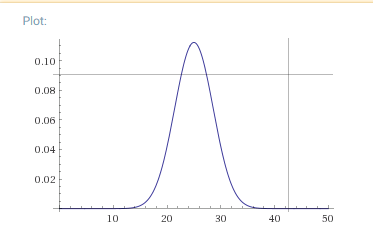
\includegraphics[width=0.5\textwidth]{./figures/FiftyCoins.png}
\end{figure}

\section*{Problem 2.5}
\subsection*{Part a}
Problem: List all microstates of an Einstein solid with $N=3,q=4$.
\\
\\
Solution: $\Omega(3,4) = \binom{4+3-1}{4} = 15$, so we expect fifteen total solutions,
which are:
\\
(4,0,0)
(0,4,0)
(0,0,4)\\
(3,1,0)
(1,3,0)
(3,0,1)\\
(1,0,3)
(0,3,1)
(0,1,3)\\
(2,2,0)
(2,0,2)
(0,2,2)\\
(2,1,1)
(1,2,1)
(1,1,2)\\

\subsection*{Part b}
What about for $N=3,q=5$?
\\
\\
Solution: $\Omega(3,5) = \binom{5+3-1}{5} = 21$, so we expect twenty one total solutions,
which are:
\\
(5,0,0)
(0,5,0)
(0,0,5)\\
(4,1,0)
(4,0,1)
(0,4,1)\\
(1,4,0)
(1,0,4)
(0,1,4)\\
(3,1,1)
(1,3,1)
(1,1,3)\\
(3,2,0)
(3,0,2)
(0,3,2)\\
(2,3,0)
(2,0,3)
(0,2,3)\\
(2,2,1)
(2,1,2)
(1,2,2)

\section*{Problem 2.6}
Problem: Calculate the multiplicity of an Einstein solid with $N=q=30$.
\\
\\
Solution: The multiplicity is $\Omega (30,30) = \binom{30+30-1}{30} \approx 5.91\times 10^{16}$.


\section*{Problem 2.7}
Problem: For an Einstein solid with four oscillators and two units of energy, represent the
states as a series of dots and lines.
\\
\\
Solution:\\
$|||\cdot\cdot$\\
$||\cdot|\cdot$\\
$||\cdot\cdot|$\\
$|\cdot|\cdot|$\\
$|\cdot||\cdot$\\
$|\cdot\cdot||$\\
$\cdot|||\cdot$\\
$\cdot||\cdot|$\\
$\cdot|\cdot||$\\
$\cdot\cdot|||$\\
%----------------------------------------------------------------------------------------

\end{document}
